\documentclass[tikz,border=12pt]{standalone}
\usepackage{amsmath,amssymb}
\usepackage{tikz}
\usetikzlibrary{arrows.meta,positioning,fit,calc}

\definecolor{qtC}{HTML}{1F4E79}
\definecolor{dqC}{HTML}{0B6E4F}
\definecolor{ink}{HTML}{1A1A1A}
\definecolor{bgSoft}{HTML}{F7F5F1}
\definecolor{midC}{HTML}{4B5563}

\begin{document}
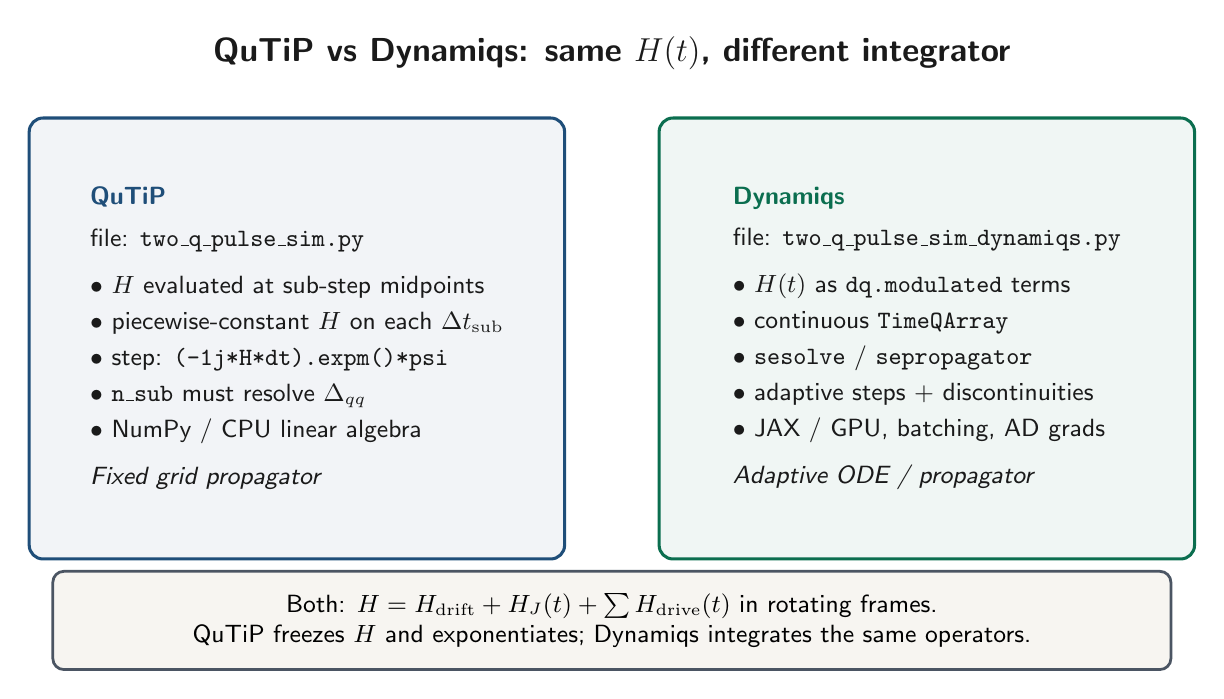
\begin{tikzpicture}[
  font=\sffamily\small,
  >={Stealth[length=2.2mm]},
  panel/.style={
    draw=#1, line width=1.1pt, rounded corners=5pt,
    fill=#1!6, align=left, inner sep=10pt, text=ink,
    minimum width=6.8cm, minimum height=5.6cm
  },
  title/.style={font=\sffamily\bfseries\large, text=ink},
  head/.style={font=\sffamily\bfseries, text=#1}
]

\node[title] at (0,4.0) {QuTiP vs Dynamiqs: same $H(t)$, different integrator};

\node[panel=qtC, anchor=north] (L) at (-4.0,3.2) {%
  {\color{qtC}\textbf{QuTiP}}\\[4pt]
  file: \texttt{two\_q\_pulse\_sim.py}\\[6pt]
  $\bullet$\ $H$ evaluated at sub-step midpoints\\[2pt]
  $\bullet$\ piecewise-constant $H$ on each $\Delta t_{\mathrm{sub}}$\\[2pt]
  $\bullet$\ step: \texttt{(-1j*H*dt).expm()*psi}\\[2pt]
  $\bullet$\ \texttt{n\_sub} must resolve $\Delta_{qq}$\\[2pt]
  $\bullet$\ NumPy / CPU linear algebra\\[6pt]
  \textit{Fixed grid propagator}
};

\node[panel=dqC, anchor=north] (R) at (4.0,3.2) {%
  {\color{dqC}\textbf{Dynamiqs}}\\[4pt]
  file: \texttt{two\_q\_pulse\_sim\_dynamiqs.py}\\[6pt]
  $\bullet$\ $H(t)$ as \texttt{dq.modulated} terms\\[2pt]
  $\bullet$\ continuous \texttt{TimeQArray}\\[2pt]
  $\bullet$\ \texttt{sesolve} / \texttt{sepropagator}\\[2pt]
  $\bullet$\ adaptive steps + discontinuities\\[2pt]
  $\bullet$\ JAX / GPU, batching, AD grads\\[6pt]
  \textit{Adaptive ODE / propagator}
};

\node[draw=midC, line width=1pt, rounded corners=4pt, fill=bgSoft,
      align=center, inner sep=8pt, minimum width=14.2cm]
  at (0,-3.2) {%
  Both: $H=H_{\mathrm{drift}}+H_J(t)+\sum H_{\mathrm{drive}}(t)$
  in rotating frames.\\
  QuTiP freezes $H$ and exponentiates; Dynamiqs integrates the same operators.
};

\end{tikzpicture}
\end{document}
